\documentclass{amsart}
\usepackage{graphicx}
\setlength{\topmargin}{-1.2cm}
\setlength{\leftmargin}{0.2cm}
\setlength{\rightmargin}{0.2cm}
\setlength{\textheight}{25.00cm} 
\setlength{\textwidth}{16.00cm}
\parindent 0pt
\parskip 3pt
\pagestyle{plain}
\begin{document}

\title{ Parity and Pigeonhole Principle}
\author{Collected by: Duttatrey N. Srivastava}
%    Remove any unused author tags.


\date{15 April 2019}

%\begin{abstract}
%\end{abstract}

\maketitle

\section{Parity}
 Given Natural Numbers(often with 0), consider its remainder when divided by 2. Parity is the property of an integer to be even (i.e. divisible by 2) or be odd (i.e. not divisible by 2). Despite the simplicity of this concept, parity can be used in showing that many arrangements are impossible to make.

\subsection{Part I: Direct problems}
\begin{enumerate}
\item Prove that the sum of 2 odd numbers or 2 even numbers is always even. Further, show that sum of an odd and an even number is always odd.
\item Generalisation: Sum of even many even numbers is even; sum of even many odd numbers is even; sum of odd many odd numbers is odd.
\item Show that if the sum of two numbers is odd, their product is always even.
\item If sum of some collection of numbers is odd, then the collection has odd-many odd numbers in it.
\item If the parity of product of certain collection of numbers is odd, then none of those numbers is even.
\end{enumerate}

\subsection{Part II:Warm up problems}
\begin{enumerate}
\item Can a $ 5 \text{x} 5$ square checkerboard be covered with $1 \text{x} 2$ dominos without spilling over?
\item 5 gears are arranged in a cycle. Can all the gears move simultaneously?
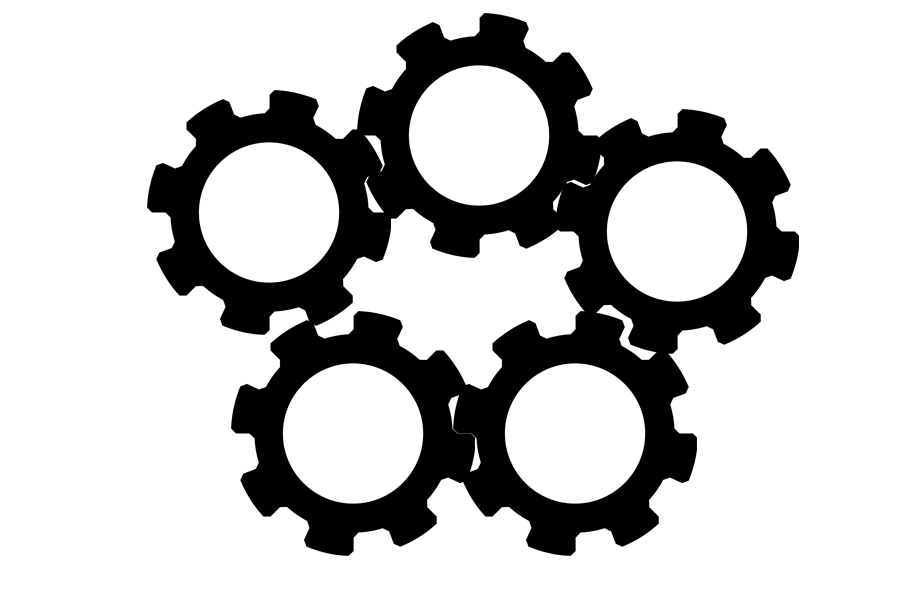
\includegraphics[scale=0.3]{gr.jpg}
\item  Suppose you have $\$25$. You want to change it using exactly $10$ bills of $\$1$ , $\$3$ , and  $\$5$. Can you possibly get the change?
\end{enumerate}

\subsection{Part III: Games and Parity}
\begin{enumerate}
\item Can a knight starting at $a1$ on a chessboard, reach the position $h8$ while visiting each of the sqaures exactly once?
\item Suppose, on a chess board, a knight is ploaced at $a1$. After several moves, the knight returns to position $a1$. Has the knight moved even number of times, or odd number of times?
\end{enumerate}

\subsection{Odd and Even}

\begin{enumerate}
\item Peter has a notebook with 96 pages(excluding covers). He numbered them $1,2,3,\ldots,192$ in order. Tony tore 25 pages from the notebook, and added the 50 numbers on them. Could tony possibly get 2020 as a sum of those page numbers?
\item The product of 22 integers is 1. Show that their sum cannot be 0.

\end{enumerate}

\subsection{General Problems}
\begin{enumerate}
\item (Hungarian Contest, 1906) Let $\{a_1,a_2,\ldots a_n\}$ be an arbitrary arrangement of numbers $1,2,\ldots,n$. Show that, given $n$ is odd, the product $$(a_1-1)(a_2-2)\ldots(a_n-n)$$
is even.
\end{enumerate}
One problem for the road:
\begin{enumerate}
\item A snail crawls along a plane with constant velocity, turning a right angle every 15 minutes. Show that the snail could return to its starting point only in whole number of hours.
\end{enumerate}


\section{Pigeonhole Principle}

\textbf{Statement:} If there are $n$ pigeonholes, and at least $n+1$ pigeons, then there is atleast one hole with atleast two pigeons.

Pf: By Contradiction: What happens if none of the holes have more than one pigeon?
\\

Usual Strategy goes like this:
\begin{enumerate}
\item Recognise that the problem requires Pigeonhole principle
\item Identify holes and pigeons.
\item Apply the principle; the problem might involve further steps, so think of this step as penultimate(just before the final step) helps.
\item Solve the problem.
\end{enumerate}
We will discuss variants and generalizations of the principle as we go along; then a couple of olympiad problems.



\subsection{Part I: Warm up Problems}

\begin{enumerate}
\item A bag has socks of two colors: white and black. What is the smallest number of socks that you need to take out(without looking) so that we surely have two socks of same colour?
\item Given $12$ integers, show that two of them can be chosen such that their difference is divisible by $11$.
\item In the movie ”Cheaper by the Dozen,” there are 12 children in the family.
	\begin{enumerate}
\item Prove that at least two of the children were born on the same day of the week.
\item Prove that at least two family members (including mother and father) are born in the same month.
\end{enumerate}
\item $1,900,000$ trees grow in a forest. it is known that each tree may have atmost $600,000$ leaves. Can we have two trees with same number of leaves? Can you say something more? 

\end{enumerate}

\subsection{A little geometry}
In many cases, the pigeonhole principle acts like the crucial final or penultimate step of the argument: Our aim should be to focus on the initial strategy and avoid pitfalls as we go about it. The important thing when beginning is to not give up immediately. 
\begin{enumerate}
\item Given a unit square and 5 points lying inside the square: show that their are 2 points which are atmost $\frac{\sqrt{2}}{2}$ units apart.
\item Every point on a plane is coloured red or blue. Prove that no matter how it is coloured, there are two points of the same color exactly 1 metre apart.
\item Prove that any equilateral triangle cannot be covered (overlap allowed) completely by 2 smaller equilateral triangles.
\end{enumerate}


\subsection{General Pigeons!}

\textbf{Statement:} If there are $n$ pigeonholes, and at least $nk+1$ pigeons, then there is atleast one hole with atleast $k+1$ pigeons.
Proof:Similar to the earlier one.
\begin{enumerate}
\item 25 crates of apples are delivered to a store. There are 3 varieties of apples:Jazz, Reds, and Green. Each crate contains exactly one type of apples. Prove that there are atleast 9 crates of the same sort of apples.
\item Ten students solved a total of $35$ problems in a math olympiad. Each problem was solved by exactly one student. There is at least one student who solved exactly one problem, at least one student who solved exactly two problems, and at least one student who solved exactly three problems. Prove that there is  also at least one student who solved at least 5 problems. 
\end{enumerate}

\subsection{Sums of some kind}

\textbf{Statement:} If there are $n$ numbers that sum up to $S$, then at least one of those numbers is smaller than $S/n$.

\begin{enumerate}
\item $5$ workers earned $\$ 1500.00$ for work during a week. Each of them wants to buy a phone that costs $\$ 310.00$ online. Show that one of them will have to wait till next week to buy the phone.
\end{enumerate}•

\subsection{Part III: A little Number Theory}
Many divisibility problems are simply clever uses of the pigeohole principle.
\begin{enumerate}
\item Show that there are two powers of two, such that their difference is divisible by 2019.
\item Show that there is a number written entirely with the digit $1$, such that the number is divisible by 2019.
\item Show that there is a power of $3$ which ends with the digits $001$.
\item(CSMO 1986) Prove that given any $n$ distinct integers, one can find a subset of the integers such that their sum is divisible by $n$.
\end{enumerate}
One problem for the road:

\begin{enumerate}

\item Consider a $10$ x $10$ chessboard. Suppose 41 rooks are placed on the board. Show that there are 5 rooks, none of which attack the other 

\end{enumerate}•
$$\circ\cup\cap\cup\cap\cup\cap\cup\cap\cup\cap \circ$$
\end{document}